\subsection{Przegląd obiecujących pętli sterowania}

Przedstawiona w poprzedniej sekcji architektura jest jedynie funkcjonalna i zawiera w sobie dużo abstrakcji. Ostateczna postać wewnętrznej zamkniętej pętli sterowania w ENI system jest jeszcze w trakcie specyfikacji. ENI w dokumencie \cite{enioverview} dokonało przeglądu istniejących, możliwych do zaaplikowania architektur zamkniętych pętli sterowania. Niniejsza praca dyplomowa chce zaproponować architekturę do modelowania oraz uruchamiania pętli w ENI System, dlatego ważne jest, aby poznać jej składowe elementy oraz \textit{workflow} przykładowych pętli. Domyślamy się, że konkretne workflow pętli będzie znane dopiero przy konkretnym wdrożeniu ENI System, a wdrożeniu będą różniły się między sobą. 

\subsubsection{OODA}
Pętla autorstwa Johna R. Boyda składa się z 4 części: "Observe", "Orient", "Decide", "Act". Stanowi podsumowanie jego myśli na temat strategi, taktyki oraz procesów decyzyjnych. John R. Boyd był pułkownikiem Sił Powietrznych USA i jednym z najbardziej wpływowych myślicieli wojskowych XX wieku. Mimo, iż był wojskowym jego koncepcja składająca się z nieustannej obserwacji, orientacji, podejmowania decyzji i działania jest kluczowa w każdej formie walki. Może być również stosowana w polityce, biznesie, życiu codziennym. Główną koncepcją jest ciągłe dostosowywanie się do zmieniających się warunków oraz podważanie istniejących założeń. Koncepcja ta świetnie nadaje się do adaptacyjnych oraz kognitywnych systemów zarządzania.

Architektura pętli OODA przedstawiona jest na rysunku \ref{fig:24-ooda}

\begin{figure}[!h]
    \centering 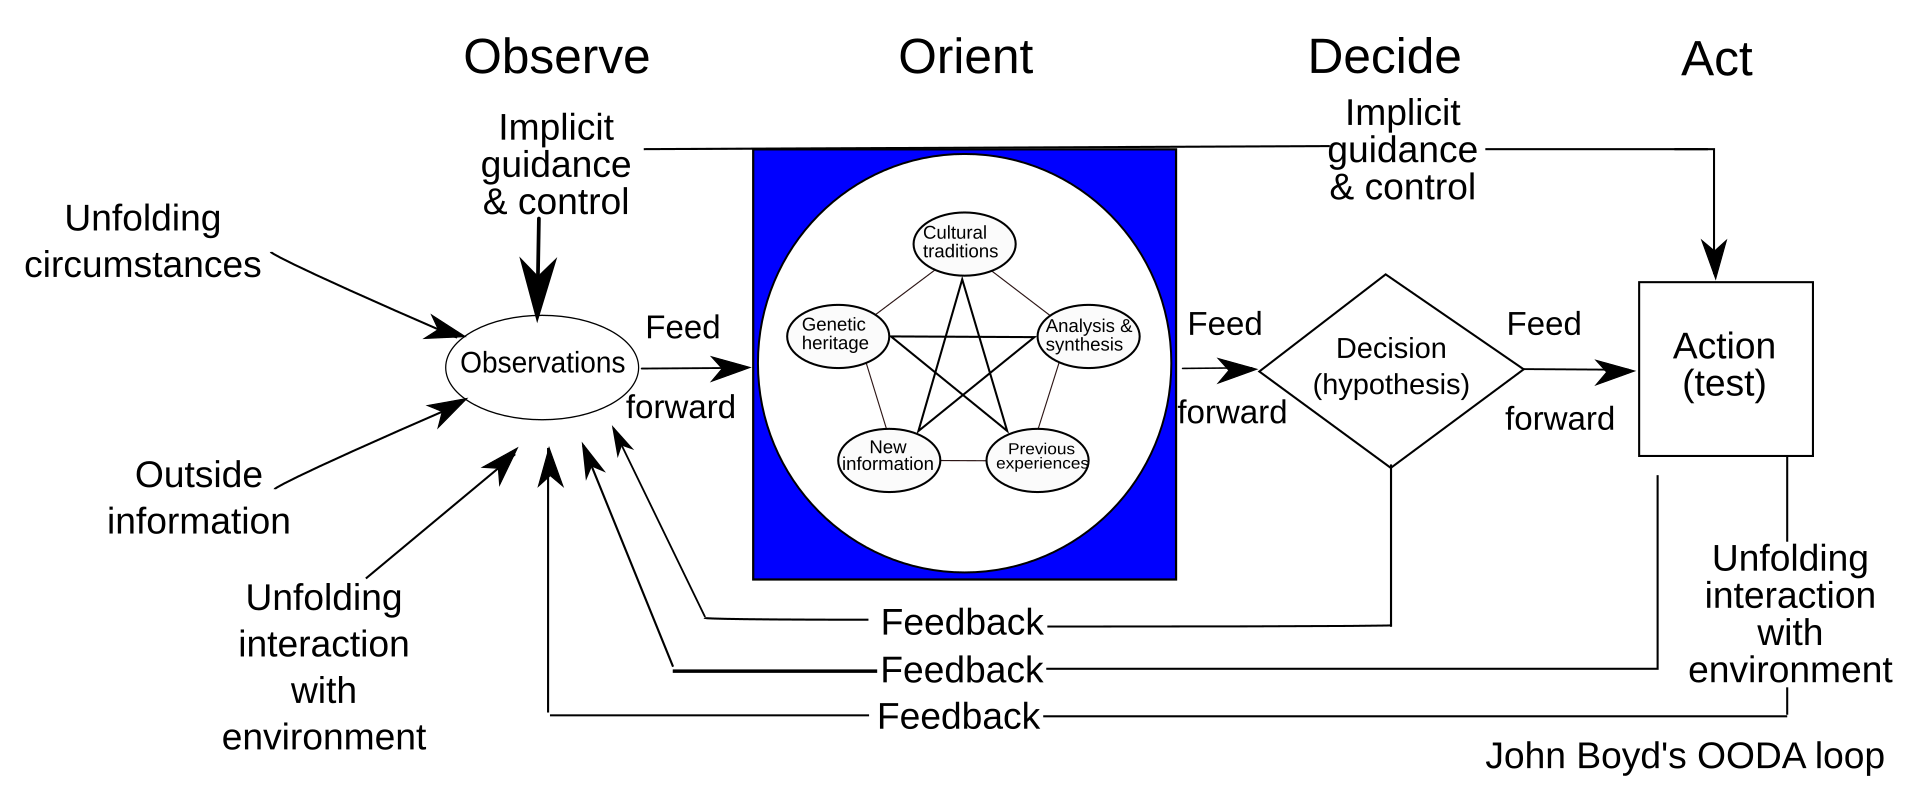
\includegraphics[width=1\linewidth]{24-ooda.png}
    \caption{Architektura pętli OODA}\label{fig:24-ooda}
\end{figure}


\subsubsection{MAPE-K}
MAPE-K jest to pętla opracowana przez IBM w dziedzinie autonomicznego przetwarzania i systemów samoadaptujących się. Głowne jej etapy to Monitorowanie, Analiza, Planowanie, Wykonanie, a każdy z nich ma dostęp do wspólnej bazy wiedzy. 

Architektura pętli MAPE-K przedstawiona jest na rysunku \ref{fig:24-mapek}

\begin{figure}[!h]
    \centering 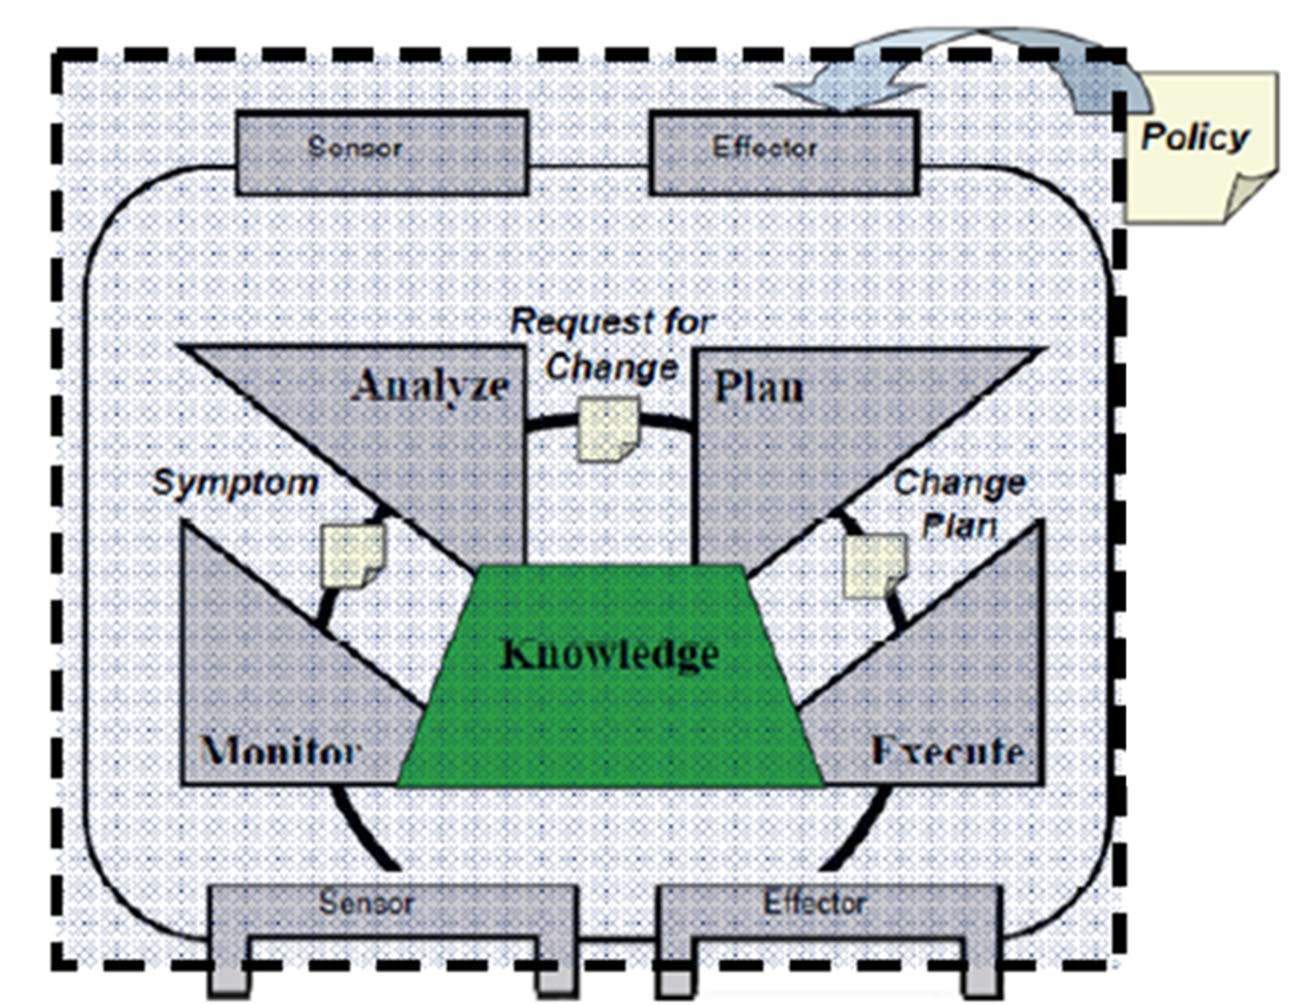
\includegraphics[width=1\linewidth]{24-mapek.png}
    \caption{Architektura pętli MAPE-K}\label{fig:24-mapek}
\end{figure}

\subsubsection{FOCALE}
Nazwa tej pętli pochodzi słów: Podstawa (ang. \textit{Foundation}), Obserwacja (ang. \textit{Observation}), Porównanie (ang. \textit{Comparison}), Analiza (ang. \textit{Analysis}), Uczenie (ang. \textit{Learning}), Wnioskowanie (ang. \textit{rEason}). Niespotykanym dotąd elementem może być Podstawa, która jest statyczną częścią modelu i określa strukturę oraz podstawowe zasady systemu. Ta architektura jako pierwsza proponuje też element odpowiedzialny za uczenie maszynowe (ang. \textit{machine learning}). 

Architektura pętli FOCALE przedstawiona jest na rysunku \ref{fig:24-focale}

\begin{figure}[!h]
    \centering 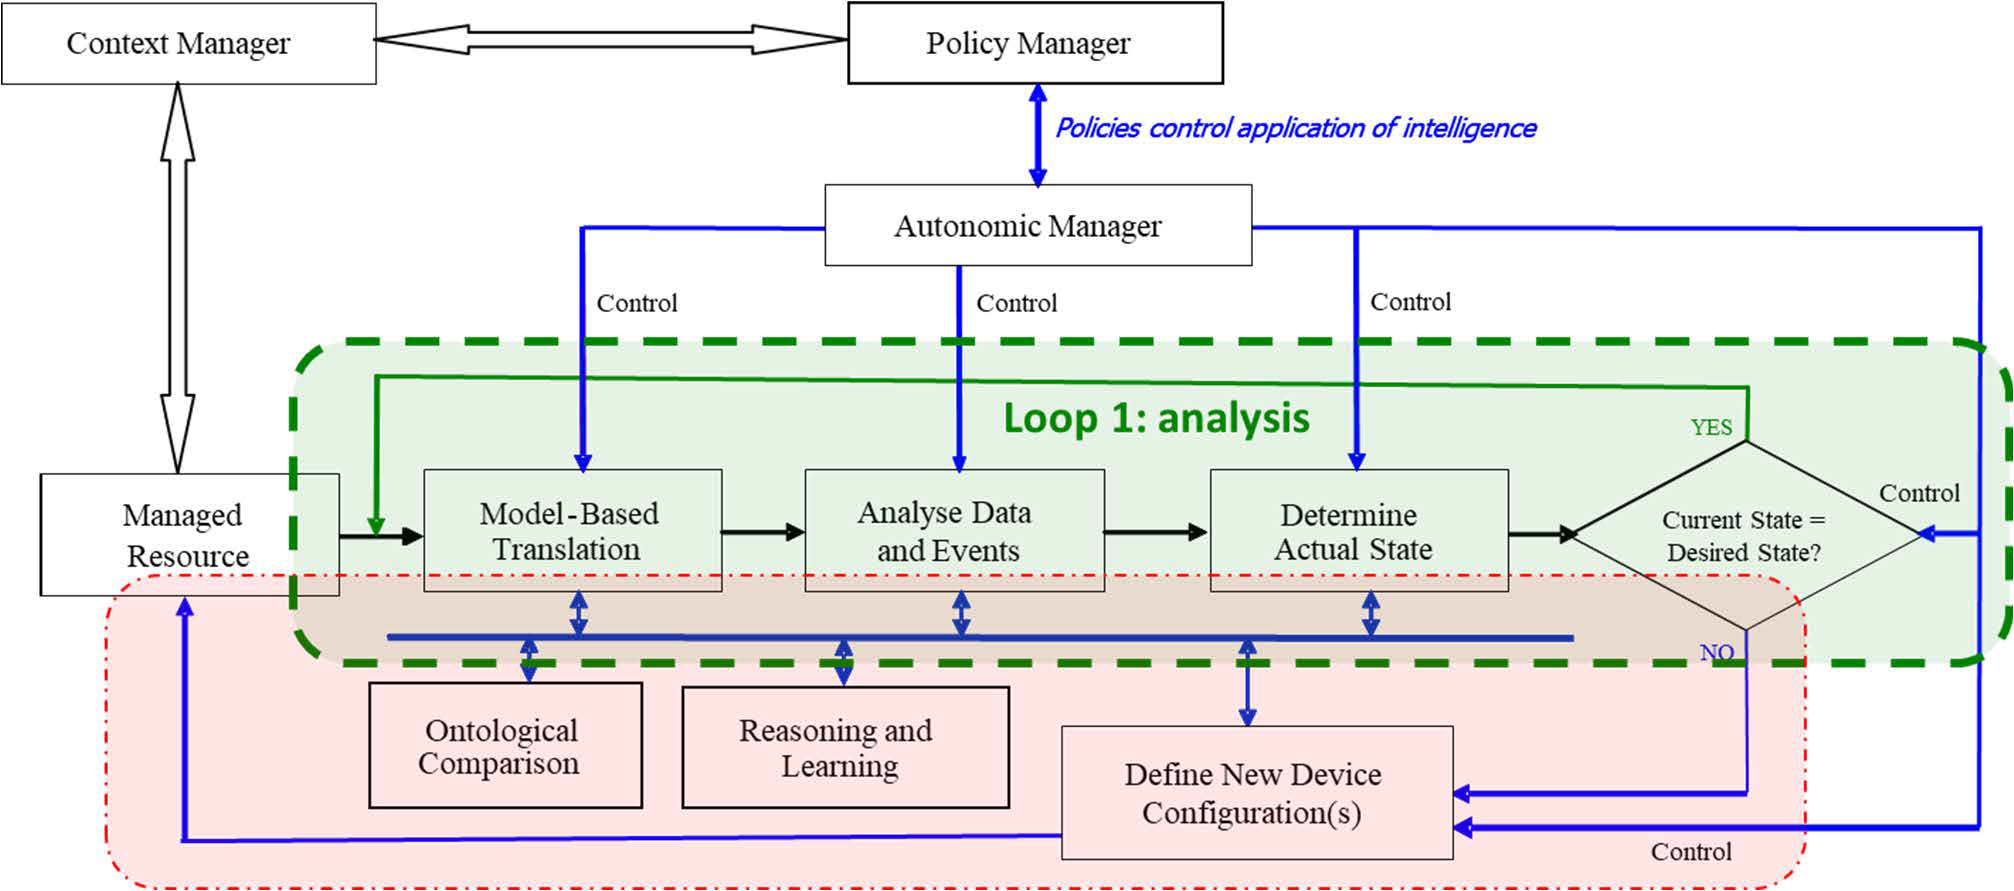
\includegraphics[width=1\linewidth]{24-focale.png}
    \caption{Architektura pętli FOCALE}\label{fig:24-focale}
\end{figure}

\subsubsection{COMPA}
Elementy tej pętli to: Analityka (ang. \textit{Analytics}), Polityki (ang. \textit{Policies}) oraz Sterowanie, Orkiestracja i Zarządzanie (ang. \text{Control, Orchestration, Management})

Architektura pętli COMPA przedstawiona jest na rysunku \ref{fig:24-compa}

\begin{figure}[!h]
    \centering 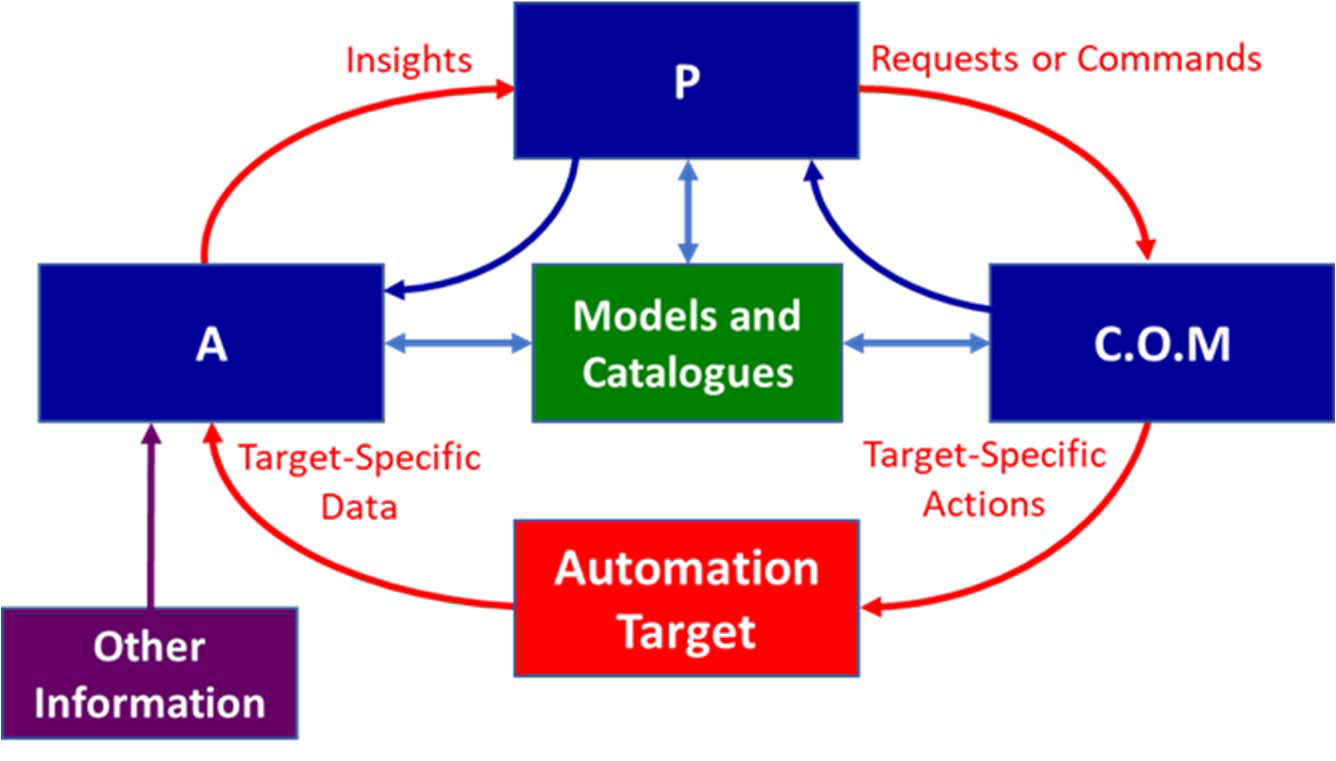
\includegraphics[width=1\linewidth]{24-compa.png}
    \caption{Architektura pętli COMPA}\label{fig:24-compa}
\end{figure}